\chapter{Periodicity and image counters}
\label{ch:periodicity}

\section{Wrapped positions and continuous coordinates}

On a periodic axis $k$ with period $L_k$ every vertex position is stored \emph{wrapped} into
$[x_{\min,k},x_{\max,k})$. A surface that crosses the periodic face is therefore stored in pieces
at both ends of the box, although it is one connected mesh. To know where each vertex lies on
the unbroken surface, every vertex carries integer \emph{image counters} \texttt{img[3]}, and its
\emph{continuous coordinate} is
\begin{equation}
  \vect{X} = \texttt{pos} + \texttt{img}\odot\vect{L},
  \label{eq:continuous}
\end{equation}
with $\texttt{img}_k=0$ on non-periodic axes. \fn{MFTLVertexContinuous} evaluates
(\ref{eq:continuous}). For vertices with large counters the library never forms $\vect{X}$ inside
sums; it uses coordinates relative to a reference vertex, with the integer part exact:
\begin{equation}
  \vect{Y} = (\texttt{img}-\texttt{img}_{\text{ref}})\odot\vect{L} + (\texttt{pos}-\texttt{pos}_{\text{ref}})
  \qquad (\fn{MFTLVertexRelative}).
\end{equation}

\section{Minimum image and the edge-length restriction}

The only geometric restriction is local: \textbf{every edge is shorter than half a period} on
every periodic axis. Then the difference of the wrapped positions of the two ends of an edge,
reduced by one period where it exceeds half a period, is the true edge vector:
\begin{equation}
  d_k(u,v) = \Delta_k - L_k\,[\Delta_k > L_k/2] + L_k\,[\Delta_k < -L_k/2],\qquad
  \Delta_k = \texttt{pos}_{v,k}-\texttt{pos}_{u,k}
  \label{eq:minimage}
\end{equation}
(\fn{MFTLGetMinimumImageVector}). Every local kernel --- triangle properties, curvature, fits,
smoothing, boundary geometry --- works with minimum-image differences from an anchor vertex, so a
triangle across a seam is treated exactly like one in the middle of the box.
\fn{MFTLCheckMinimumImageConstraint} (collective) checks the edge restriction; there is no
restriction on the size of a body.

\section{Keeping the counters right}
\label{sec:displacement}

The counters stay meaningful because every vertex update follows one \emph{displacement rule}:
a vertex moves by a displacement shorter than half a period from an anchor with a known
continuous coordinate, and the new position is wrapped with the wrap counted into
\texttt{img}. The helpers in \texttt{mftl\_geometry.h} implement the cases:
\begin{description}
  \item[\fn{MFTLWrapPosImg}\texttt{(dom, pos, img)}] wraps a position that moved by less than one
    period and counts the wrap: $\texttt{pos}\mathrel{-}=L_k$, $\texttt{img}_k\mathrel{+}=1$ above the box,
    and the reverse below. The continuous coordinate is unchanged.
  \item[\fn{MFTLImgFollow}\texttt{(dom, img, old, new)}] updates the counters when a wrapped position
    is \emph{replaced} by an independently wrapped value (a fit, a smoothing result): the move is
    taken as the minimum-image displacement.
  \item[\fn{MFTLWrapContinuous}\texttt{(dom, X, pos, img)}] turns a continuous input coordinate
    into $(\texttt{pos},\texttt{img})$ with $\texttt{img}_k=\lfloor (X_k-x_{\min,k})/L_k\rfloor$.
  \item[\fn{MFTLWrapObjectIntoDomain}\texttt{(obj)}] wraps all owned vertices of a body, counting
    every wrap.
\end{description}
\fn{MFTLApplyPeriodicity} wraps a bare point (for example a query point); it must not be used on
a vertex, because it does not count the wrap.

Table~\ref{tab:imglife} lists how the library maintains the counters.

\begin{table}[ht]
\centering\small
\begin{tabularx}{\textwidth}{@{}lX@{}}
\toprule
Event & Counter rule \\
\midrule
Continuous input (generators, GTS files) & $\texttt{img}=\lfloor(\vect{X}-\vect{x}_{\min})\oslash\vect{L}\rfloor$, then canonicalisation \\
Wrapped input without counters (native v1 files, soups) & $\texttt{img}=0$, then canonicalisation assigns consistent counters \\
Translation by the application or \fn{MFTLTranslateObject} & positions move without wrapping; \fn{MFTLWrapObjectIntoDomain} wraps and counts \\
Scaling, rotation (\fn{MFTLScaleObject}, \fn{MFTLRotateObject}) & continuous coordinates relative to the body reference point, then wrap \\
Split of an edge $a\to b$ & the new vertex is placed from anchor $a$ by the minimum-image displacement \\
Collapse, fits, smoothing, volume recovery & displacement rule from the vertex's own anchor \\
Flip & no vertex changes \\
Redistribution, ghost refresh & \texttt{img} travels with \texttt{pos} \\
Native mesh v2 / restart & stored and restored exactly \\
\bottomrule
\end{tabularx}
\caption{Lifecycle of the image counters.}
\label{tab:imglife}
\end{table}

\section{Winding and canonicalisation}
\label{sec:winding}

\paragraph{Edge lattice shift.} For an edge $u\to v$ and a periodic axis $k$, the integer
\begin{equation}
  s_k(u,v) = \operatorname{round}\!\left(\frac{X_{v,k}-X_{u,k}-d_k(u,v)}{L_k}\right)
  = \texttt{img}_{v,k}-\texttt{img}_{u,k}+j_k,
  \label{eq:shift}
\end{equation}
where $j_k\in\{-1,0,1\}$ is the wrap in (\ref{eq:minimage}), measures how many periods the
continuous coordinates jump along the edge (\fn{MFTLEdgeShift}). An edge with $s_k\neq0$ is a
\emph{cut edge} along $k$.

\paragraph{Winding.} Around any closed cycle $\gamma$ of mesh edges the minimum-image
displacements add up to the true displacement around the cycle, which is $L_k W_k(\gamma)$ with
\begin{equation}
  W_k(\gamma) = \sum_{e\in\gamma} s_k(e).
\end{equation}
A connected component \emph{winds} (wraps) along $k$ if some cycle has $W_k\neq0$ --- the surface
closes on itself only after going once (or more) around the period. This is a topological
property of the embedded surface; it does not depend on the values of the counters. A sphere
across a seam does not wind; a ribbon spanning the box along $x$ winds along $x$; a flat film
spanning $x$ and $y$ winds along both (Figure~\ref{fig:winding}).

\begin{figure}[ht]
\centering
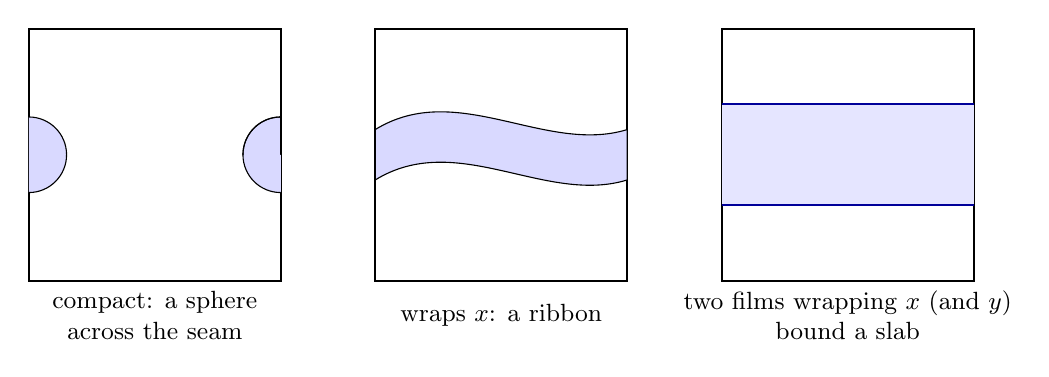
\begin{tikzpicture}[scale=0.8]
  \begin{scope}
    \draw[thick] (0,0) rectangle (4,4);
    \draw[fill=blue!15] (4,2) ++(-0.6,0) arc (180:90:0.6) -- (4,2.6) -- (4,1.4) arc (-90:-180:0) -- cycle;
    \fill[blue!15] (3.4,2) arc (180:270:0.6) -- (4,2) -- cycle;
    \draw (4,2.6) arc (90:270:0.6);
    \fill[blue!15] (0,2.6) arc (90:-90:0.6) -- cycle; \draw (0,2.6) arc (90:-90:0.6);
    \node[font=\small,align=center] at (2,-0.55) {compact: a sphere\\ across the seam};
  \end{scope}
  \begin{scope}[xshift=5.5cm]
    \draw[thick] (0,0) rectangle (4,4);
    \draw[fill=blue!15] (0,1.6) .. controls (1.3,2.4) and (2.7,1.2) .. (4,1.6) -- (4,2.4) .. controls (2.7,2.0) and (1.3,3.2) .. (0,2.4) -- cycle;
    \node[font=\small,align=center] at (2,-0.55) {wraps $x$: a ribbon};
  \end{scope}
  \begin{scope}[xshift=11cm]
    \draw[thick] (0,0) rectangle (4,4);
    \fill[blue!10] (0,1.2) rectangle (4,2.8);
    \draw[blue!60!black,thick] (0,1.2) -- (4,1.2); \draw[blue!60!black,thick] (0,2.8) -- (4,2.8);
    \node[font=\small,align=center] at (2,-0.55) {two films wrapping $x$ (and $y$)\\ bound a slab};
  \end{scope}
\end{tikzpicture}
\caption{Compact and wrapping bodies in a periodic box (cross-sections).}
\label{fig:winding}
\end{figure}

\paragraph{Canonicalisation} (\fn{MFTLCanonicaliseImages}, collective). Pieces of a mesh that
were supplied independently (a soup from several ranks, a file, an assembly of components) may
carry counters in inconsistent \emph{gauges}: correct continuous positions modulo the lattice, but
with artificial cut edges between pieces. Canonicalisation removes them:
\begin{enumerate}
  \item the edge graph with its shifts is gathered on rank 0;
  \item per connected component a deterministic breadth-first spanning tree from the smallest
    vertex id defines a potential $\varphi$ with $\varphi(\text{root})=0$ and
    $\varphi(v)=\varphi(u)+s(u,v)$ along tree edges;
  \item the counters become $\texttt{img}'=\texttt{img}-\varphi$: positions are unchanged and every
    continuous coordinate moves by a whole lattice vector, so it is the same physical point;
    tree edges now have zero shift, and a non-tree edge keeps the residual
    $r(e)=s(e)-(\varphi(v)-\varphi(u))$, the winding of its fundamental cycle;
  \item the root keeps its counter (whole-body re-gauge), so the body stays where it was;
  \item the per-axis \emph{wrap flags} are cached: $\texttt{wrap}_k=1$ iff some residual has
    $r_k\neq0$.
\end{enumerate}
After canonicalisation cut edges exist only where the surface genuinely winds. The builders,
readers and generators canonicalise; the remesher preserves the winding (its operations are
short and anchored). \fn{MFTLObjectEnsureWinding} canonicalises a body whose state is unknown
(it is called by every operation that depends on the class), and \fn{MFTLObjectRegaugeImages}
brings every root counter to zero.

\section{Body classes}
\label{sec:classes}

\begin{lstlisting}[numbers=none]
int MFTLObjectWrapFlags(const MFTL_Object *obj, int wrap[3]); /* cached flags */
int MFTLObjectIsCompact(const MFTL_Object *obj);  /* compact on every periodic axis */
int MFTLObjectHasVolume(const MFTL_Object *obj);  /* closed and compact */
int MFTLObjectReference(const MFTL_Object *obj, double pos_ref[3], int img_ref[3]);
int MFTLCountCutEdges(MFTL_Object *obj, int count[3]);
\end{lstlisting}
A body is \textbf{compact} along a periodic axis when it does not wind along it; its continuous
coordinates along that axis are then globally consistent, whatever its extent. A body that is
closed and compact on every axis encloses a volume by itself, and the single-body integrals of
Chapter~\ref{ch:geometry} apply. A body that wraps a periodic axis, or is open, does not enclose a
volume by itself; its closed-phase quantities are defined only as part of a phase-boundary set
(Chapter~\ref{ch:phasesets}). \fn{MFTLObjectTakeClassTransition} reports (once) that the last
canonicalisation changed a body's wrap flags --- for example after a coalescence that joined a
body with its own periodic image.

The \emph{body reference point} (\fn{MFTLObjectReference}, collective) is the continuous
coordinate of the vertex with the lowest global id; the integrals are formed relative to a
collectively agreed anchor vertex in this way, which keeps them exact for bodies far from the
origin image.
